\documentclass{article}
\usepackage[utf8]{inputenc}

\title{MATH2710 — Portfolio 1.5 - 2.3}
\author{Mike Medved}
\date{February 8th, 2023}

\usepackage{color}
\usepackage{amsthm}
\usepackage{amssymb} 
\usepackage{amsmath}
\usepackage{lmodern}
\usepackage{mathtools, nccmath}
\usepackage{listings}
\usepackage[margin=1in]{geometry} 
\usepackage[table,xdraw,dvipsnames]{xcolor}
\usepackage{tikz}

\usepackage{xparse}
%
\DeclarePairedDelimiterX{\set}[1]{\{}{\}}{\setargs{#1}}
\NewDocumentCommand{\setargs}{>{\SplitArgument{1}{;}}m}
{\setargsaux#1}
\NewDocumentCommand{\setargsaux}{mm}
{\IfNoValueTF{#2}{#1} {#1\,\delimsize|\,\mathopen{}#2}}%{#1\:;\:#2}

\parindent = 0pt

\newtheorem*{thm}{Theorem}

\begin{document}

\maketitle

\section{Sets}

\subsection{Set Union}

The union of two sets $A$ and $B$ is the set of all elements that are in $A$ or $B$ or both. For two sets, $A$ and $B$ this is denoted by $A \cup B$.

$$A \cup B = \{x \in \mathbb{R} | x \in A \text{ or } x \in B\}$$

$\hfill \break$
Similarly, the union of a family of sets, $(A_i)_i$, is denoted by $\bigcup A_i$ and contains elements from all sets in the family such that $x \in A_i$ for some $i$.

$$\bigcup A_i = \{x \in \mathbb{R} | x \in A_i \text{ for some } i\}$$

\subsection{Set Intersection}

The intersection of two sets $A$ and $B$ is the set of all elements that are in both $A$ and $B$. For two sets, $A$ and $B$ this is denoted by $A \cap B$.

$$A \cap B = \{x \in \mathbb{R} | x \in A \text{ and } x \in B\}$$

$\hfill \break$
Similarly, the intersection of a family of sets, $(A_i)_i$, is denoted by $\bigcap A_i$ and contains elements from all sets in the family such that $x \in A_i$ for all $i$.

$$\bigcap A_i = \{x \in \mathbb{R} | x \in A_i \forall i\}$$

\subsection{Set Difference}

The difference of two sets $A$ and $B$ is the set of all elements that are in $A$ but not in $B$. For two sets, $A$ and $B$ this is denoted by $A \setminus B$.

$$A \setminus B = \{x \in \mathbb{R} | x \in A \text{ and } x \notin B\}$$

\subsection{Symmetric Difference}

The symmetric difference of two sets $A$ and $B$ is the set of all elements that are in $A$ or $B$ but not both. For two sets, $A$ and $B$ this is denoted by $A \triangle B$.

$$A \triangle B = \{x \in \mathbb{R} | x \in A \text{ or } x \in B \text{ but not both}\}$$

\subsection{Distributive Property}

\begin{thm}
Let $A$, $B$, and $C$ be sets. Then the following are equivalent:

$$A \cap (B \cup C) \equiv (A \cap B) \cup (A \cap C)$$
$$A \cup (B \cap C) \equiv (A \cup B) \cap (A \cup C)$$
\end{thm}

\subsection{Compliments}

Let $U$ be a non-empty set, referred to as the Universal Set. Let $A \subseteq U$, we can say that the complimentary of $A$ with respect to $U$ is the set $U \setminus A$, denoted as $A^c$.

$\hfill \break$
Visually, the compliment $A^c$ can be represented as the slashed area in Figure 1:

\begin{figure}[!htb]
    \centering
    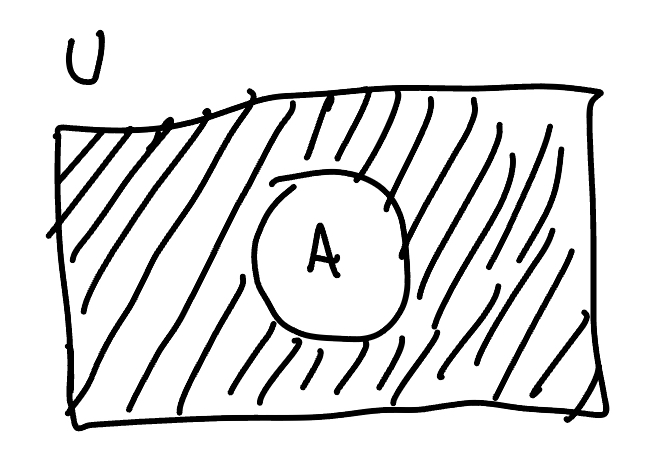
\includegraphics[scale=0.125]{./set-compliment.jpeg}
    \caption{Set Compliment}
    \label{fig:set-compliment}
\end{figure}

\subsection{De Morgan's Laws}

\subsubsection{$\left(A \cup B\right)^c \equiv A^c \cap B^c $}

De Morgan's Law states that the compliment of the union of two sets is equivalent to the intersection of the compliments of the two sets. Visually, this is represented below.

\begin{figure}[!htb]
    \centering
    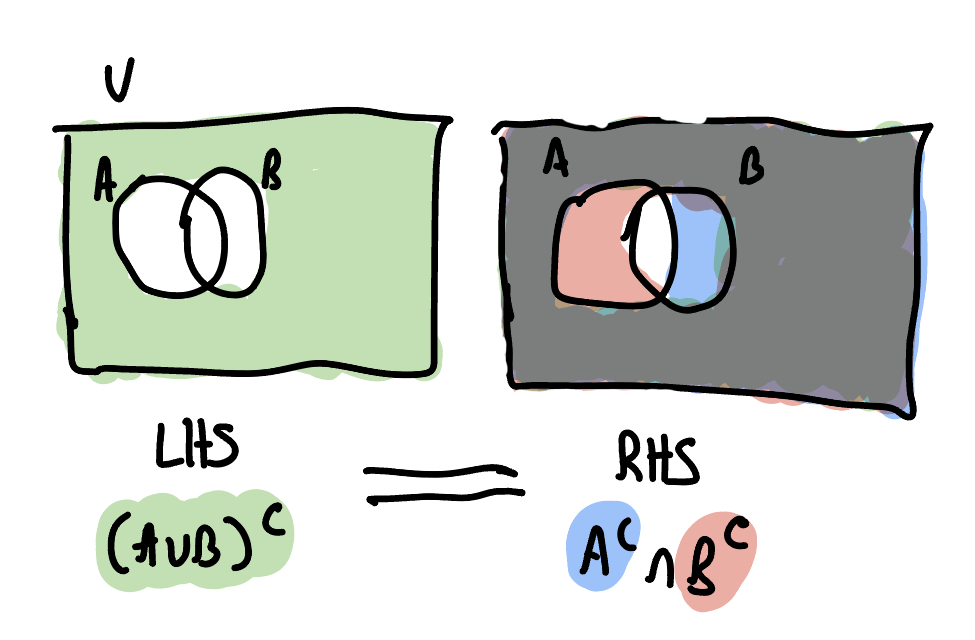
\includegraphics[scale=0.125]{./demorgans-1.jpeg}
    \label{fig:demorgans-1}
\end{figure}

\subsubsection{$\left(A \cap B\right)^c \equiv A^c \cup B^c $}

De Morgan's Law also states that the compliment of the intersection of two sets is equivalent to the union of the compliments of the two sets. Visually, this is represented below.

\begin{figure}[!htb]
    \centering
    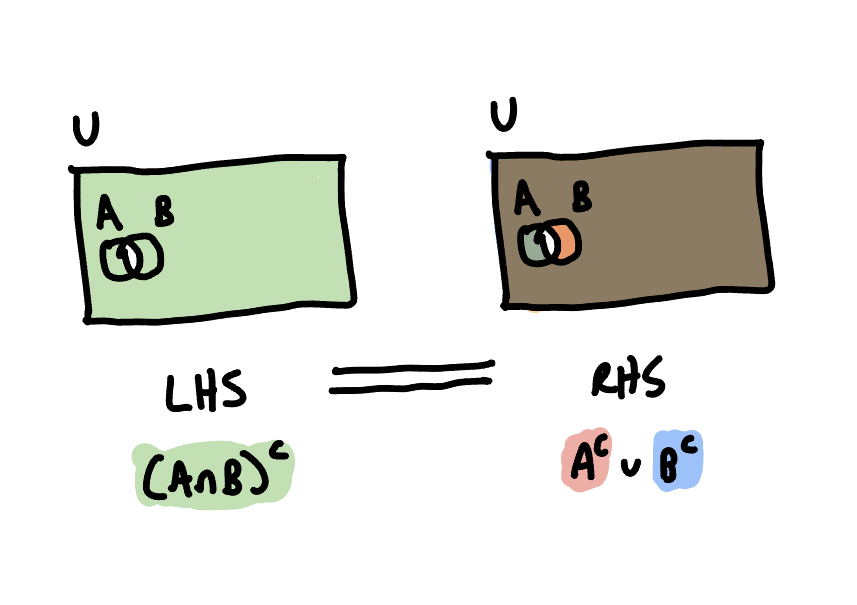
\includegraphics[scale=0.175]{./demorgans-2.jpeg}
    \label{fig:demorgans-2}
\end{figure}

\newpage
\subsection{Complimentary Example}

The below is an example in which the compliment of $A$ is intersected with the disk $B$. Specifically, $A$ is a rectangle bounded by $[0, 2] \times [0, 4]$, and $B$ is a disk centered at $(0, 0)$ with radius $2$. Further, $A^c \cap B$ is represented by the orange shaded area in Figure 3.

\begin{figure}[!h]
    \centering
    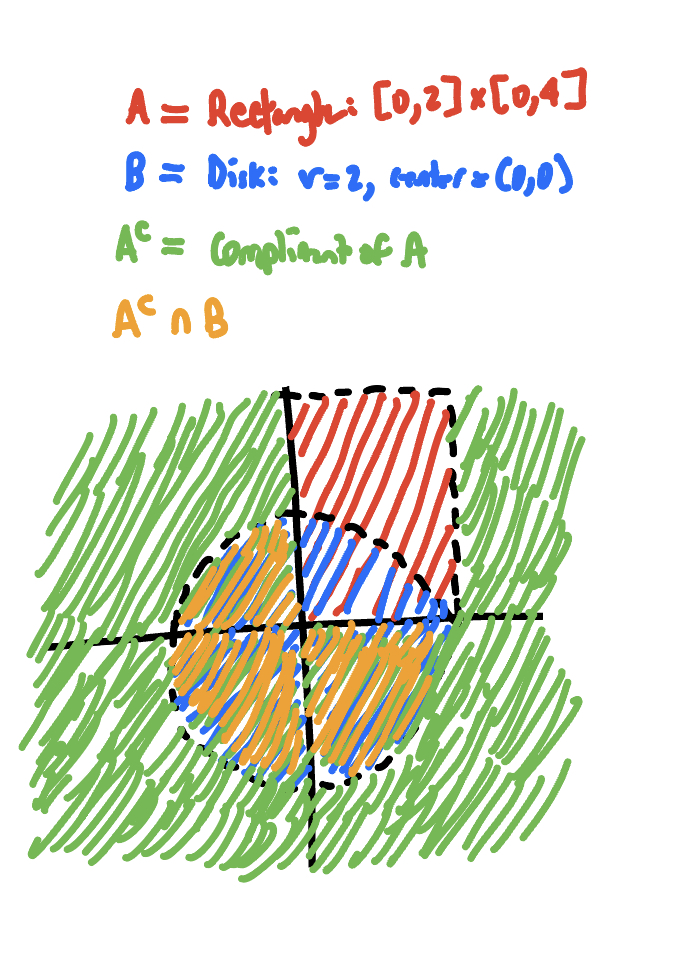
\includegraphics[scale=0.25]{./compliment.jpeg}
    \caption{Complimentary Example}
    \label{fig:complimentary-example}
\end{figure}

\subsection{Partitions}

The partition of a non-empty universal set $U$ is a family of non-empty subsets of $U$ such that both (a) the union of these subsets is $U$, and (b) the sets are mutually disjoint.

\subsubsection{Examples}

\begin{enumerate}
    \item Split $U = \left\{1, 2, 3, 4, 5\right\}$ into a partition. One possible partition is $A_1 = \left\{1, 2, 3\right\}, A_2 = \left\{4\right\}, A_3 \left\{5\right\}$. This is a valid partition because the union of the sets is $U$ and the sets are mutually disjoint. Further, we can freely arrange the sets $A_i$ in any order with any amount of elements such that there are $A_i$ $1 \leq |i| \leq 5$ subsets $A_i$ totalling at most 5 elements.
    \item Split $\mathbb{R}$ into a partition. As there is an infinite number of ways to arrange an infinite number of elements, there are an infinite number of partitions of $\mathbb{R}$. We will choose a common one of these partitions, such that $A_1 = \left\{0, 2, 4, 6, 8, \ldots\right\}, A_2 = \left\{1, 3, 5, 7, 9, \ldots\right\}$. In this way, we are partitioning the set of reals into even and odd numbers, respectively $A_1$ and $A_2$.
\end{enumerate}

\newpage
\section{Statements}

The difference between an open sentence and a statement is the fact that statements are definitely \textit{true} or \textit{false}, whereas open sentences are \textit{true} for some values of variables that are involved, but \textit{false} for others. 

$\hfill \break$
For example, the open sentence $x > 0$ is \textit{true} for $x = 1$, but \textit{false} for $x = -1$. However, the statement that the number $2 \in \mathbb{R}$ is \textit{true} regardless. Similarly, the statement that $-1 \in \mathbb{N}$ is \textit{false} regardless.

\subsection{$P$ and $Q$: $P \land Q$}

The statement $P \land Q$ is only true when both values for $P$ and $Q$ are \textit{true}, as shown in the below truth table.

\begin{table}[!htb]
    \centering
    \begin{tabular}{|c|c|c|}
        \hline
        \textbf{P} & \textbf{Q} & \textbf{P $\land$ Q} \\ \hline
        \rowcolor[HTML]{67FD9A} 
        T          & T          & T                             \\ \hline
        F          & F          & F                             \\ \hline
        T          & F          & F                             \\ \hline
        F          & T          & F                             \\ \hline
    \end{tabular}
\end{table}

\subsection{$P$ or $Q$: $P \lor Q$}

The statement $P \lor Q$ is true when either $P$ or $Q$ are \textit{true}, as shown in the below truth table.

\begin{table}[!htb]
    \centering
    \begin{tabular}{|c|c|c|}
        \hline
        \textbf{P} & \textbf{Q} & \textbf{P $\lor$ Q} \\ \hline
        \rowcolor[HTML]{67FD9A} 
        T          & T          & T                             \\ \hline
        F          & F          & F                             \\ \hline
        \rowcolor[HTML]{67FD9A} 
        T          & F          & T                             \\ \hline
        \rowcolor[HTML]{67FD9A} 
        F          & T          & T                             \\ \hline
    \end{tabular}
\end{table}

\subsection{Either $P$, or $Q$: $P \oplus Q$}

The statement Either $P$, or $Q$ - otherwise named the ``Exclusive Or" (XOR) - is true when either $P$ or $Q$ are \textit{true}, but not both. This is shown in the below truth table.

\begin{table}[!htb]
    \centering
    \begin{tabular}{|c|c|c|}
        \hline
        \textbf{P} & \textbf{Q} & \textbf{P $\oplus$ Q} \\ \hline
        T          & T          & F                             \\ \hline
        F          & F          & F                             \\ \hline
        \rowcolor[HTML]{67FD9A} 
        T          & F          & T                             \\ \hline
        \rowcolor[HTML]{67FD9A} 
        F          & T          & T                             \\ \hline
    \end{tabular}
\end{table}

\newpage
\subsection{If $P$, then $Q$: $P \Rightarrow Q$}

The statement If $P$, then $Q$ is true for all values such that $P = Q$ or $\lnot P = Q$. This statement type can be thought of as a type of promise, where $P$ is the promise and $Q$ is the result of the promise. Let's say that the promise $P$ is that you take the final exam for a class, the result $Q$ is that you pass the class. If you take the final exam, you will pass the class. If you do not take the final exam, you will not pass the class. The only value that does not hold true is when you take the final exam and fail the class. This is shown in the below truth table.

\begin{table}[!htb]
    \centering
    \begin{tabular}{|c|c|c|}
        \hline
        \textbf{P} & \textbf{Q} & \textbf{P $\Rightarrow$ Q} \\ \hline
        \rowcolor[HTML]{67FD9A} 
        T          & T          & T                             \\ \hline
        \rowcolor[HTML]{67FD9A} 
        F          & T          & T                             \\ \hline
        T          & F          & F                             \\ \hline
        \rowcolor[HTML]{67FD9A} 
        F          & F          & T                             \\ \hline
    \end{tabular}
\end{table}

\subsubsection{Sufficiency and Necessity}

When it is stated "$P$ is a sufficient condition for $Q$," it is saying that if $P$ is true, then $Q$ is true. Similarly, when it is stated "$Q$ is a necessary condition for $P$," it is saying that if $Q$ is true, then $P$ is must be true.

\subsubsection{Hypothesis and Conclusion}

The hypothesis for the statement "$P \Rightarrow Q$" is $P$, and the conclusion is $Q$.

\subsubsection{Converse}

The converse of the statement "$P \Rightarrow Q$" is "$Q \Rightarrow P$".

\subsubsection{Example}

An example of a statement that is true for both it's regular and converse forms:

\begin{itemize}
    \item $P \Rightarrow Q:$ If $t$ is an equilateral triangle, then $t_1 = t_2 = t_3$ where $t_i$ represents the $i$th side. \textbf{(T)}
    \item $Q \Rightarrow P:$ If $t_i$ represents the $i$th side and $t_1 = t_2 = t_3$, then the triangle $t$ is equilateral. \textbf{(T)}
\end{itemize}

Furthermore, an example of a statement that is true for it's regular form, but \textit{false} for it's converse form:

\begin{itemize}
    \item $P \Rightarrow Q:$ If $f$ is continuous on $[a, b]$, then it is Riemann Integrable on $[a, b]$. \textbf{(T)}
    \item $Q \Rightarrow P:$ If $f$ is Riemann Integrable on $[a, b]$, then it is continuous on $[a, b]$. \textbf{(F)}
\end{itemize}

\end{document}